\section{Training and Creating the Model}
\label{sec:formatting}

We modeled our original model from a previous submission on Kaggle created by Emmanuel Pintelas, training the model using ResNets and transfer learning. 
The final accuracy with three epochs was 81.9\%. Between our three memembers, we split modification of the model into error analysis \& split protocol, convolution networks \& saturation, and development of non-neural networks.

%-------------------------------------------------------------------------
\subsection{Split Protocol}

All data was split based on the provided 26 drivers, using 70\% of the set for training, and the final 30\% for testing validation.
The split was based on previous industry reports\cite{maDigitalTwin2024} on the best split for their training model and became the basis for ours.
A random image level split allows any duplicate frames of the same driver taken from the original videos in both the training and testing data for confirmation.
Using \verb+GroupShuffleSplit+ with \verb+subject+ as the group, 200 candidate seeds with the split seed DEFINE created a held-out fraction near 30\% where all ten classes appear and chosen for performance.
The final split uses NUMBER drivers for training (15,703 images) and NUMBER drivers for testing (6,721 images) with confirmation that the sets are disjoint.



%-------------------------------------------------------------------------
\subsection{Error Analysis}

Error analysis included metrics not previously shown for the model to help better determine accuracy, bias, as well as allow us to be able to determine the best modifications for finetuning.
New statistics included: entropy loss, F1 precision, and total accuracy. These were accomplished by using sklearn metrics to be computed after and during the model.

Originally, the model did not fair the best with an accuracy of 51.8\%. 
Recall was the highest with the driver operating the radio at 0.91, and steadily declined from mid 0.6 in makeup, texing, and reaching behind range down to 0.16 when talking to the passenger.
Based on how similar some of the poses are such as texting and using the phone, the recall is a significantly higher due to the clusters it creates by similarity.

The largest issue that can be denoted from this data is the inability to generalize new drivers.
Not only is this denoted in the accuracy, but the high cross entropy.

\begin{figure}[t]
  \centering
    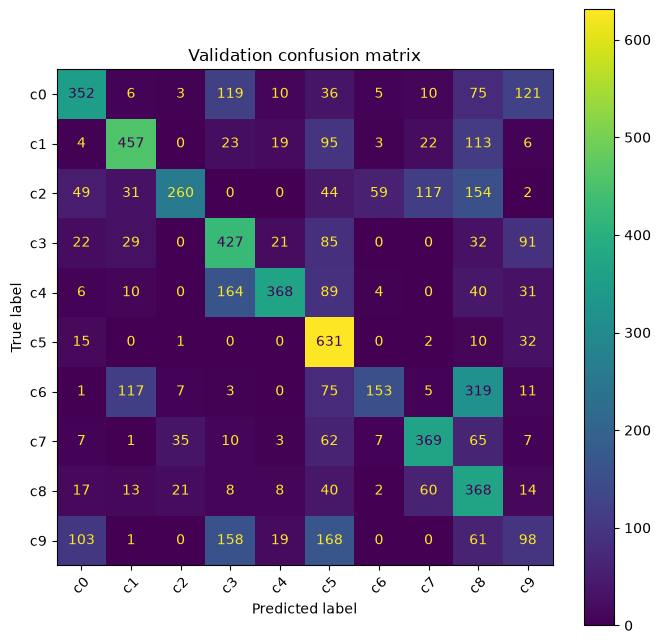
\includegraphics[width=\linewidth]{figures/Val_Conf_Matrix.png}
    \caption{Original confusion matrix after training.}
    \label{ffig:confmat}
  \hfill
\end{figure}

